\documentclass{article}
\usepackage{verbatim,pgfgantt,graphicx}
\PassOptionsToPackage{hyphens}{url}\usepackage{hyperref}
\begin{document}
\title{Interim Report}
\author{Michael Sledge\\ CN:121677}
\date{}
\maketitle
\section{Introduction}
Distributed systems can have many useful applications as they allow easy scalability and higher reliability due to the lack of a single point of failure when compared to standalone systems. Distributed hash tables are a way of building distributed systems using independent, self-organising nodes using methods much like a hash table, i.e. key, value pairs.  A DHT consists of a keyspace to which everything is mapped, a partition scheme which maps keys to nodes and an overlay network to allow each node to find the node to which a particular key is assigned. The key hashing and partitioning scheme must be such that with no change in nodes, keys map to the same node and a node leaving or arriving only affects its two adjacent nodes.

DHTs and similar distributed systems are widely used in many well-known large dynamic web applications for a range of purposes, primarily performance improvements for content fetching and the scalability and availability they provide.

DHTs are fully decentralised so that responsibility for maintaining the network is spread over all nodes and the effects of failures of individual nodes a can be minimised, this also has several other advantages: a DHT can be scaled to an extremely large number of nodes with little to no change in the design of nodes themselves, functionality can be maintained even when the availability of individual nodes fluctuates.

An important aspect of maintaining scalability and performance of network applications is the way network I/O is handled. There are two ways of handling multiple connections simultaneously: synchronously, where a new thread or process is created for each connection, this method is fairly simple but also scales poorly as large numbers of connections will require a large number of threads, leading to much overhead from context switching; and asynchronously, which allows a single thread to handle many connections by initiating I/O operations then continuing to do other processing tasks such as dealing with completed I/O operations while waiting for the I/O to complete.

The aim of this project will be to produce tools for building distributed systems based on DHTs with high network performance and scalability with use of asynchronous I/O. It should involve implementing DHT functionality for nodes allowing users to implement the functionality to be distributed on a network.

This report will cover professional and ethical considerations, related research and systems, more detailed technical requirements, and a record of phases which have been completed and those still to be completed.

\section{Professional Considerations}
The BCS Code of Conduct [1] sets out the following standards which may be relevant to this project: 2 c) “develop your professional knowledge, skills and competence on a continuing basis, maintaining awareness of technological developments, procedures, and standards that are relevant to your field.” and 2 d) “ensure that you have the knowledge and understanding of Legislation* and that you comply with such Legislation, in carrying out your professional responsibilities.”

From ‘Professional Competence and Integrity’ in Annex A Interpretation of the BCS Code of Conduct [2]: “You should seek out and observe good practice exemplified by rules, standards, conventions or protocols that are relevant in your area of specialism.”

Existing libraries may be used in this project and their licenses must be followed, standards and conventions in languages used should be followed also.



\section{Background Reading/Existing solutions}
The chord protocol [3] uses consistent hashing to assign keys to nodes. It defines a set of functions which nodes use to build and maintain a chord network. Chord nodes in a network form a virtual ring in which each node is aware of its immediately adjacent nodes as well as several succeeding nodes.
Nodes are mapped into the same keyspace used for identifiers for the application
Each node knows how to find the node that an identifier maps to, illustrated in fig 1. If the id is between the current node and its successor then it maps to the successor, otherwise it asks the furthest node it knows about that is not past the id in the keyspace. The succeeding nodes that a node has knowledge of are stored in a 'finger' table (illustrated as dashed arrows in fig 1.) These are not necessary for functionality but they reduce the number of steps when mapping a key to a node.
\begin{figure}
\centering
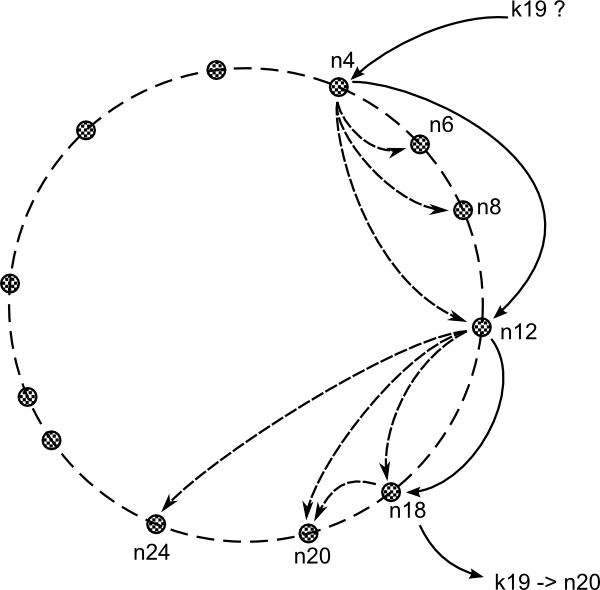
\includegraphics{chord_find-successor.png}
\caption{Finding the successor for key 19. Dashed arrows show which nodes a node has knowledge of (some have been omitted for clarity).}
\end{figure}

The stabilisation that chord nodes run periodically is important to keep the network functional as the availability of nodes changes. Stabilisation is executed as follows: the node checks if there is a node between itself and its recorded successor, if there is it updates its recorded successor; then the node notifies its recorded successor of its existence so it can update its predecessor record if necessary. Nodes also periodically update their finger tables, and check whether their predecessor is still accessible.
\begin{figure}
\centering
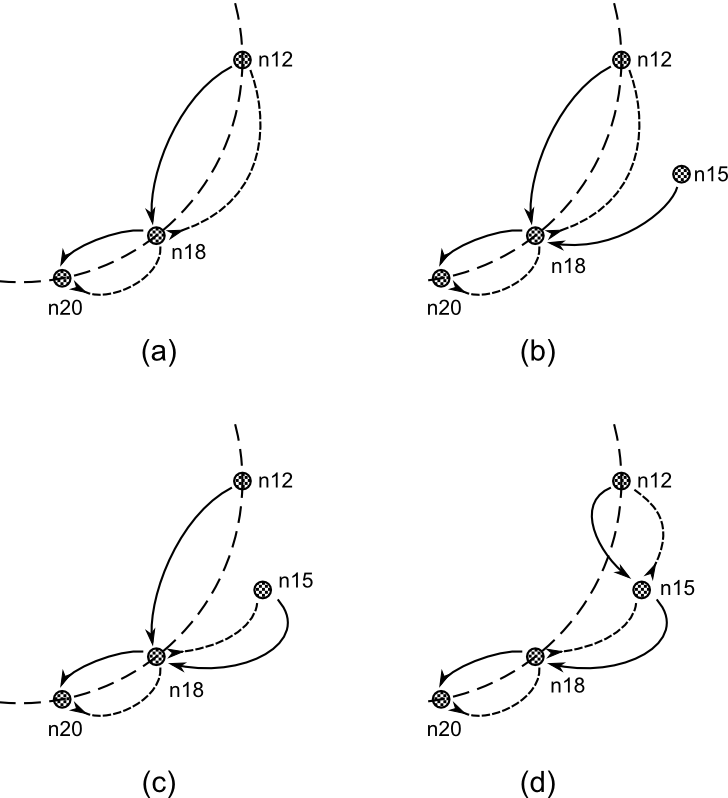
\includegraphics{chord_joining.png}
\caption{Node joining and stabilisation. (a) A chord network in a stable state. (b) new node n15 joins having found its successor (c) n15 runs its stabilisation and now n18 is aware of n15. (d) n12 runs its stabilisation and the network is back to as stable state}
\end{figure}
\\
\\
Memcached [4] is a distributed in-memory caching system based on a distributed hash table intended for use in speeding up web applications by caching database entries, though it is possible to use it for other similar purposes. It is used by many large web companies.

Memcached uses spare memory on web servers to create a distributed in-memory cache which can be used to alleviate server load. This provides several benefits when compared to having each server managing it's own individual cache: the combined cache is much larger than individual caches; cached data is consistent any server requesting the a key in the cache will get the same value, whereas separate caches may not update data at the same time; improved scalability, as more servers are added to handle increasing load the size of the cache increases, making large scaling much easier than it would be with individual caches per server.
\\
\\
Mace [5] is a toolkit for building distributed systems which “seeks to transform the way distributed systems are built by providing designers with a simple method for writing complex but correct and efficient implementations of distributed systems.” [6] It is designed to provide a common 'language' to design distributed systems without having to implement the entire system from scratch, it provides and uses libraries to build systems. The restrictions mace imposes in this way allow for better options for debugging a distributed system.

Nodes in mace are made up of one or more layers and each layer is built on an event driven state machine. Like Chord, Mace creates a virtual overlay network in which each node keeps a record of adjacent nodes, periodically updating these records and notifying the application when changes occur.
\\
\\
Libevent [7] is a cross platform C library which provides a single API for implementing event driven network servers using one of a number of mechanisms systems provide for event notification, to allow for asynchronous I/O operations. Libevent checks for events and runs the callbacks specified for each event in the queue. An event can be a notification for a socket becoming read- or write-able, a new connection on a listen socket or a timer event among other things. Libevent also provides bufferevents to simplify the task of using read and write buffers with socket events. Libevent also includes a simple HTTP, DNS and RPC (remote procedure call) implementations.
\\
\\
Similar to Libevent, Boost.Asio [8] is a cross platform C++ library providing a consistent API for network and low level I/O programming with an asynchronous model. Its scope is slightly narrower than libevent's, so it doesn't include the simple protocol implementations.
\section{Requirements Analysis}
Build a high performance library for building DHT based systems with asynchronous I/O for scalability. Nodes should be independent and self organising, requiring no central authority, and be tolerant of joining leaving and failing of nodes in the system.

Functional requirements:
\begin{itemize}
\item
Creating and joining a network
\item
Finding the node a key maps to from any node on the network.
The algorithm finds the node a key maps to directly or finds the next hop and passes the job of finding it on to that node.
\item
Periodic stabilisation to account for change in availability of nodes.
Periodic checking for failures of adjacent nodes and arrival of new nodes. New nodes must notify at least one node of their presence.
\item
Allow sending of messages or data to other nodes for the application.
Once the node a key maps to has been found allow data to be sent to that node.
\item
Provide callbacks for the application when a message is received.
Allow the application programmer to provide functions which are called when specific events occur.
\item
Provide callbacks for notifying the application of changes in the availability of nodes that may affect it, i.e. the next and previous nodes. Specifically when the set of keys a node is responsible for changes.
\end{itemize}


Non-functional requirements:
\begin{itemize}
\item
Provide high performance network communication between nodes
\item
Be highly scalable both in terms of number of nodes and the load of individual nodes assuming the application is able to handle such loads.
\end{itemize}

\section{Project Plan}


\hspace*{-3cm}
\begin{ganttchart}[hgrid,vgrid]{1}{22}
%labels
\gantttitle{Autumn}{12}
\gantttitle{Spring}{10} \\
\gantttitle{1}{1}
\gantttitle{2}{1}
\gantttitle{3}{1}
\gantttitle{4}{1}
\gantttitle{5}{1}
\gantttitle{6}{1}
\gantttitle{7}{1}
\gantttitle{8}{1}
\gantttitle{9}{1}
\gantttitle{10}{1}
\gantttitle{11}{1}
\gantttitle{12}{1}

\gantttitle{1}{1}
\gantttitle{2}{1}
\gantttitle{3}{1}
\gantttitle{4}{1}
\gantttitle{5}{1}
\gantttitle{6}{1}
\gantttitle{7}{1}
\gantttitle{8}{1}
\gantttitle{9}{1}
\gantttitle{10}{1}\\
%tasks
\ganttbar{first task}{1}{2} \\
\ganttbar{Proposal}{2}{3} \\
\ganttbar{Interim Report}{6}{7} \\
\ganttbar{Implementing network I/O}{8}{9} \\
\ganttbar{Implementing overlay network}{9}{11} \\
\ganttbar{Implementing example applications}{12}{14} \\
\ganttbar{Testing and Evaluation}{14}{16} \\
\ganttbar{Draft Report}{16}{19} \\
\ganttbar{Pesentation Poster}{18}{19} \\
\ganttbar{Final Report}{20}{22}

%relations 
\ganttlink{elem1}{elem2}
\ganttlink{elem3}{elem4}
\ganttlink{elem4}{elem5}
\ganttlink{elem5}{elem6}
\ganttlink{elem7}{elem9}
\end{ganttchart}
\hspace*{-3cm}

\section{Interim Log}
2015-09-24 initial meeting\\
2015-10-02 Meeting: discussion regarding async I/O
	Researching async I/O implementations in the form of libraries or server software such as libevent, boost::asio, node.js\\
2015-10-15 Meeting: discussion on whether a web server would be interesting and challenging in the right way and suggestions of alternatives.\\
2015-10-22 Meeting: introduction of DHTs
	Researching DHT’s more in depth \\
2015-10-30 Meeting: discussing DHTs and contents of this report
\section{Appendices}
\subsection{References}
\begin{itemize}
\item[1] BCS Code of Conduct: \url{http://www.bcs.org/category/6030}  [accessed 2015-11-01]

\item[2] BCS Code of Conduct, Annex A, Interpretation of the BCS Code of Conduct \url{http://www.bcs.org/content/ConWebDoc/39988}  [accessed 2015-11-01]

\item[3] Chord: A Scalable Peer-to-Peer Lookup Protocol for Internet Applications Ion Stoica, Robert Morris, David Liben-Nowell, David R. Karger, M. Frans Kaashoek, Frank Dabek, and Hari Balakrishnan, Member, IEEE, IEEE/ACM TRANSACTIONS ON NETWORKING, VOL. 11, NO. 1, FEBRUARY 2003

\item[4] Memcached \url{http://memcached.org/}

\item[5] Mace: Language Support for Building Distributed Systems,Charles Killian, James W. Anderson, Ryan Braud, Ranjit Jhala, Amin Vahdat

\item[6] Mace + Distributed Systems HOWTO, James W. Anderson, Charles Killian, Amin Vahdat, June 30, 2009

\item[7] Libevent \url{http://libevent.org/} [accessed 2015-11-02]

\item[8] Boost.Asio \url{http://www.boost.org/doc/libs/1_59_0/doc/html/boost_asio.html} [accessed 2015-11-04]


\end{itemize}
\subsection{Project Proposal}


\end{document}